\chapter{Content Mapping}

\label{appendix:content.mapping}

A map based approach inspired by Harry Beck's London Underground tube
map, introduced to the information
architecture field by \citet{walsh07}, will be used for visualizing the
navigational relationships between content items.
\begin{figure}[h]
  \begin{center}
    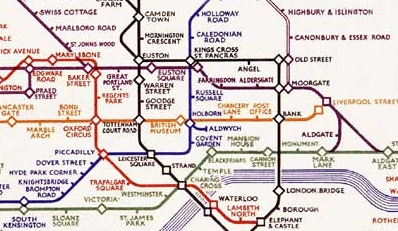
\includegraphics[width=0.9\textwidth]{beck_1933_map}
    \caption[1933 London Underground Tube map]{%
      The present Underground Tube map of London was introduced as ealy as
      1933 by graphic designer Harry Beck. It's merrits are discussed
      in ref mit, ref acm}
  \end{center}
\end{figure}

No maps are available yet since the author don't have access to the required
\emph{Adobe Illustrator} software.
